\begin{multicols}{3}[\section{C-Netz}]

\rhead{Autor: Daniel Keilmann}
\lfoot{Letzte Bearbeitung: 16.04.2016}

\newrefsegment

\begin{boxedminipage}{\linewidth}
\begin{tabular}{p{2,1 cm}p{2.7 cm}}
\textbf{Steckbrief}& \\
\end{tabular}
\begin{tabular}{p{2,1 cm}|p{2.7 cm}}
      Einsatz seit & 01.05.1985\\
      \hline
      Funkkanäle & 287 (ab 1991)\\
      \hline
      Verbreitung & DE, PT und ZA\\
      \hline
      Auslastung & 850.000 Teilnehmer\\
      \hline
      Eingestellt & 31.12.2000\\
\end{tabular}
\end{boxedminipage}
\par

\subsection*{Überblick}
Das C-Netz der DeTeMobil war seit Mitte 1984 verfügbar und startete offiziell im September 1985. Ende 2000 wurde der Betrieb eingestellt. \enquote{Anders als beim B-Netz betrieben die Nachbarländer Netze mit einem anderen technischen Standard, sodass die deutsche Form des C-Netzes nur noch in Portugal und Südafrika genutzt wurde.}~\cite{c-netz.1}\\
Zu dem Thema C-Netz wird auf die folgenden Aspekte eingegangen:
\begin{itemize}
	\item Technische Erläuterung
	\begin{itemize}[label={}]
		\item In diesem Abschnitt wird die technische Umsetzung des C-Netzes untersucht.
	\end{itemize}	
	\item Vergleich zum A- und B-Netz 
	\begin{itemize}[label={}]
		\item Hier werden die technischen Unterschiede von dem C-Netz zum A- und B-Netz dargelegt.
	\end{itemize}
	\item Einsatz		
	\begin{itemize}[label={}]
		\item Wo das C-Netz verwendet wird und wieweit es von den Bürgern benutzt wird.
	\end{itemize}
	\item Anbieter und Gremien
	\begin{itemize}[label={}]
		\item Wer das C-Netz zur Verfügung stellt.
	\end{itemize}
	\item Historische Entwicklung
	\begin{itemize}[label={}]
		\item Entwicklung des C-Netzes.
	\end{itemize}
	\item Ausblick
	\begin{itemize}[label={}]
		\item Was noch mit dem C-Netz realisiert wird und welche Folgetechnologien eingesetzt wurden.
	\end{itemize}
\end{itemize}
\subsection*{Technische Erläuterungen}

\begin{boxedminipage}{\linewidth}
\begin{tabular}{p{2,1 cm}p{2.7 cm}}
\textbf{Frequenzbereich}~\cite{c-netz.1} & \\
\end{tabular}
\begin{tabular}{p{2,1 cm}|p{2.7 cm}}
      Unterband  & \SI{451,30}-\SI{455,74}{\mega\hertz}\\
      \hline
      Oberband  & \SI{461,30}-\SI{465,74}{\mega\hertz}\\
\end{tabular}

\begin{tabular}{p{2,1 cm}p{2.7 cm}}
\textbf{Sendeleistung}& \\
\end{tabular}
\begin{tabular}{p{2,1 cm}|p{2.7 cm}}
      Feststation & max. \SI{25} Watt\\
      \hline
      Teilnehmer & max. \SI{15} Watt\\
\end{tabular}
\end{boxedminipage} \\
\\ Eine flächendeckende Versorgung wurde in Großzellen (Radius von 15-20 km) und Kleinzellen (2–3 km) in den Ballungsräumen realisiert. In den Anfangsjahren bestand das C-Netzes aus zwei Funkvermittlungsstellen und 175 Funkzonen, beziehungsweise Funkfeststationen. Das C-Netz konnte (im Endausbau) 850.000 Teilnehmer aufnehmen. Aktivierte Funkverbindungen wurden beim Wechsel der Funkzelle weitergereicht (Handover). Der C-Netz-Teilnehmer hatte im gesamten Versorgungsbereich eine einheitliche Zugangskennzahl (0161) und Funkrufnummer über die er erreichbar war. Mängel des C-Netzes waren die begrenzte Teilnehmeranzahl des C-Netzes, vergleichsweise geringe Sprachqualität und das hohe Abhörrisiko. Durch die Sprachverschleierung sollte das Abhörrisiko verringert werden, führte aber lediglich eine Invertierung des Sprachbandes aus. Dies kann mit geringen technischen Mitteln umgangen werden. Bei schlechten Verbindungen konnte der Benutzer diese ausschalten und damit die Verständlichkeit erhöhen.
Das C-Netz-System unterstützte als erstes System die Trennung von Teilnehmeridentität und Endgerät. Die Teilnehmeridentität bzw. die Zugangsberechtigung waren auf einer Magnetkarte codiert. Das heißt, durch Einschieben dieser Karte wurde ein beliebiges Mobiltelefon einem Nutzer zugeordnet. 1988 wurde der Magnetstreifen durch die TeleKarte mit integriertem Mikrocontroller ersetzt. Dies ist der Vorläufer der heute verwendeten SIM-Karte.
\begin{Figure}
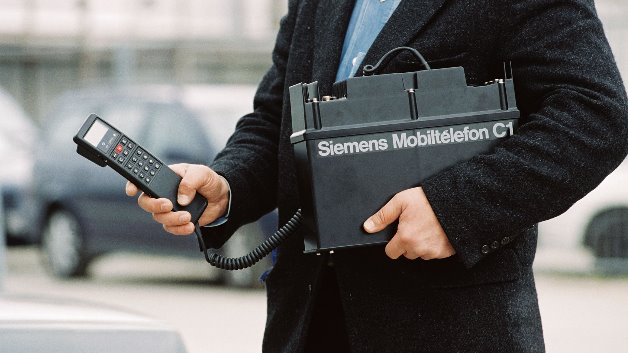
\includegraphics[width=\linewidth]{Kapitel/C-Netz/Grafiken/MobiltelefonC1.jpg}
\captionof{figure}{Mobiltelefon~\cite{c-netz.2}}
\label{fig:c-netz.mobiltelefonEins}
\end{Figure}
Für die damalige Zeit ungewöhnlich waren auch die funktional reich bestückten Hörer, die alle Bedienelemente, LC-Display und LEDs besaßen. 
Das Tastenset war gemäß der CCITT-Empfehlungen aufgebaut und die weitere Mensch-Maschine-Schnittstelle war nach einer FTZ-Richtlinie für alle Hersteller geregelt, so dass der Nutzer keine gerätespezifischen Umstellungsschwierigkeiten hatte, sondern grundsätzlich Zustände wie „eingebucht“, „verbunden“ oder „Sprachverschleierung eingeschaltet“ in bekannter Form angezeigt bekam.

Die Übertragung von Signalisierungsdaten, wurde realisiert durch die Unterteilen des Audiosignals in jeweils 12,5 ms lange Audioblöcke und deren 10 prozentige, zeitliche Kompression, um in die so entstandenen 1,25 ms langen Lücken 4-Bit-Datentelegramme einzufügen.

\subsection*{Vergleich zum A- und B-Netz}
Das C-Netz bot im Vergleich zu den dahin bekannten analogen Mobilnetzen eine Handover-Funktion, die nicht nach der Feldstärke gesteuert wurde, sondern von der relativen Entfernung zur Basisstation. Damit waren Hand-over auch schon unter besten Funkbedingungen möglich, was bei der Netzplanung und der Verdichtung der Frequenzwiederholung ein sehr nützliches Merkmal war. Auch wurde damit die Gleichkanalstörwahrscheinlichkeit deutlich reduziert. Um die relative Entfernungsmessung unterstützen zu können, war jedoch zusätzlicher technischer Aufwand nötig, nämlich eine zeitliche Synchronisation aller Basisstationen zueinander. Für das Realisieren auf Bundesebene bzw. für das Netz, besaß jede Basisstation spezifische Sender und Empfänger für Synchronisationssignale.
Gegenüber dem A-Netz und B-Netz gab es im C-Netz viele „bahnbrechende“ Neuerungen, die heute längst selbstverständlich sind z. B.:
\begin{itemize}
	\item Gemeinsame Vorwahl (0161-) für alle Mobil-Teilnehmer. Man braucht im Gegensatz zum A- und B-Netz nicht mehr zu wissen, wo sich der Teilnehmer aufhält.
	\item Unterbrechungsfreier Wechsel von einer Funkstation zur nächsten (Handover)
	\item Verschleierung des (analogen) Funksignals erschwert unberechtigtes Abhören
	\item Neben fest eingebauten Geräten auch herausnehmbare oder sogar tragbare Geräte möglich
	\item Bis zu 850.000 Teilnehmer (A-Netz 10.500, B-Netz 27.000)
	\item Seit Ende 1990 Anrufbeantworter und Ruf-umleitung als Netzmerkmal (bis dahin nur als Hardware-Zubehör)~\cite{c-netz.3}
\end{itemize}

\subsection*{Einsatz}
Das C-Netz (Funktelefonnetz-C) war ein analoges, zellulares Mobilfunknetz der deutschen DeTeMobil. Es war die dritte und gleichzeitig auch letzte analoge Generation des Mobilfunks, das als System nur in Deutschland, Portugal und Südafrika eingesetzt wurde. Die sehr gute Netzabdeckung von fast 100 Prozent machte das C-Netz zu einer sehr komfortablen Alternative zu den bisherigen Netzen. Das C-Netz wurde primär für telefonische Kommunikationsanwendungen (Autotelefonnetz) mit Zugang zum Telefonnetz und ISDN konzipiert. Das C-Netz wurde vorwiegend für Autotelefone, Küstenschiffe und Eisenbahntelefone benutzt~\cite{c-netz.1}.
Am 31. Dezember 1988 gab es bundesweit bereits 98.762 und im Land Berlin 2.076 C-Netz-Teilnehmer~\cite{c-netz.3}.
\begin{Figure}

\includegraphics[width=\linewidth]{Kapitel/C-Netz/Grafiken/C-Netz_Logo.png}
\captionof{figure}{Logo des C-Netzes~\cite{c-netz.4}}
\label{fig:c-netz.logo}
\end{Figure}
Der Betrieb des C-Netzes wurde am 31. Dezember 2000 eingestellt~\cite{c-netz.6}.

\subsection*{Anbieter und Gremien}
Das C-Netz wurde in Deutschland ausschließlich von der Telekom zur Verfügung gestellt, die dies im Auftrag des Deutschen Staates umsetzte. Zu den Telefonherstellern gehören unter anderem: 
\begin{itemize}
	\item AEG
	\item Bosch
	\item Nokia
	\item Siemens
\end{itemize}
und noch viele andere~\cite{c-netz.5}.

\end{multicols}
\newpage
\section*{Historische Entwicklung}
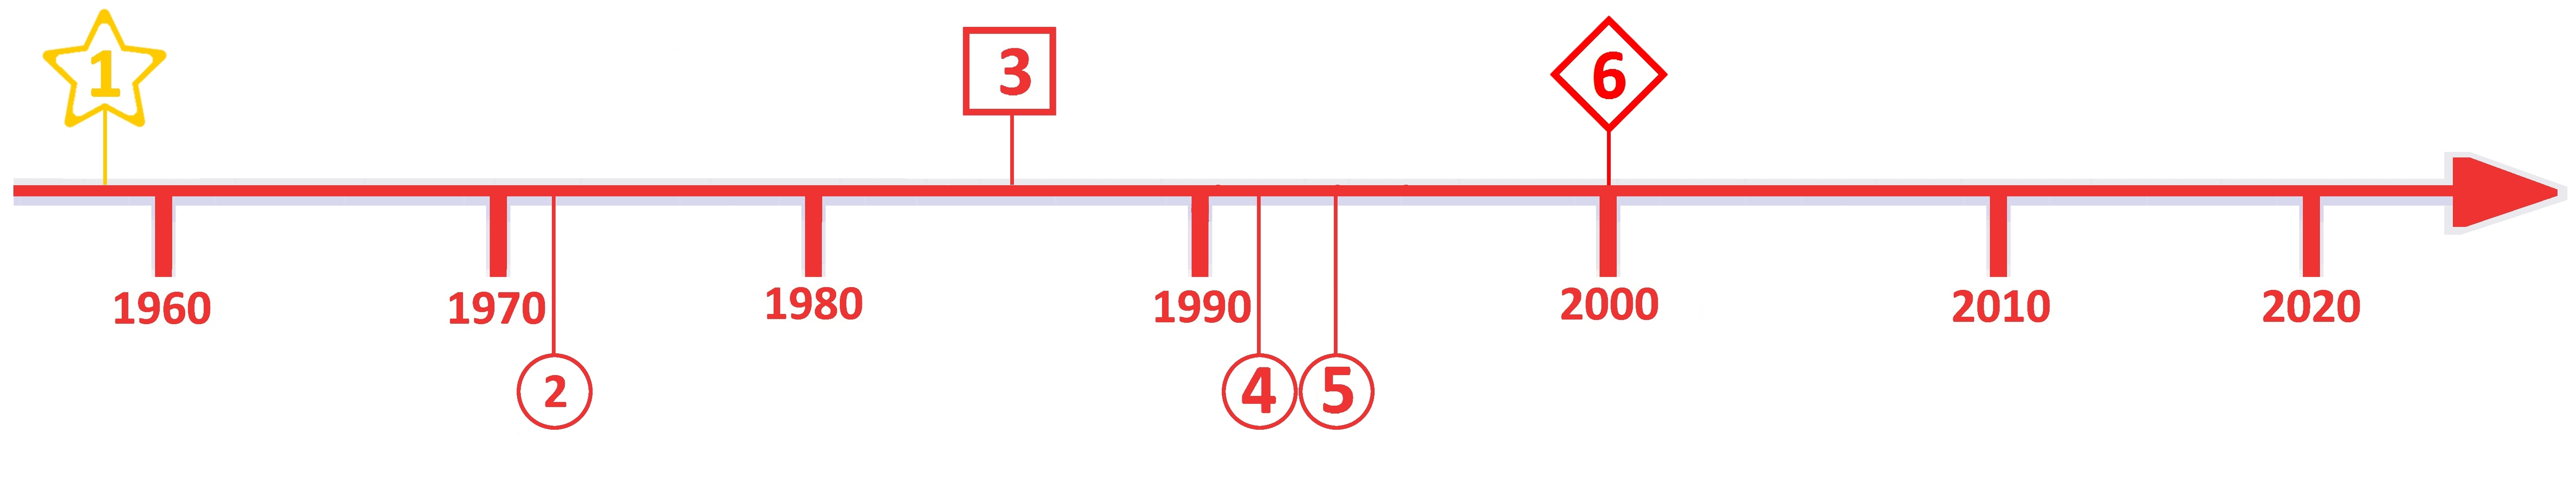
\includegraphics[width=\textwidth]{Kapitel/C-Netz/Grafiken/Zeitstrahl}
\par
\noindent
\begin{tabular}{|p{1 cm}|p{1 cm}|p{15.55 cm}|}
	\hline
	Nummer & Datum & Entwicklungsschritte~\cite{c-netz.7}\\
	\hline
	1 & 1958 & Inbetriebnahme des A-Netzes bis 1977 durch die Bundespost (daraus ging unter anderem die Deutsche Telekom hervor).\\
	\hline
	2 & 1972 & Inbetriebnahme des B-Netzes bis 1994. \\
	\hline
	3 & 1985 & DeTeMobil stellt offiziell das C-Netz zur Verfügung. In Betrieb bis 31.12.2000.\\
	\hline
	4 & 1992 & Deutsche Telekom startet offiziell das D-Netz.\\
	\hline
	5 & 1993 & E-Plus startet das E-Netz.\\
	\hline
\end{tabular}
\par
\begin{multicols}{3}
Das C-Netz wurde im Jahre 1984 (offiziell 1985) in Deutschland eingeführt und ersetzte die umständliche Handhabung des B- bzw. B2-Netzes (Fräulein vom Amt/manueller Verbindungsaufbau). Es war auf Deutschland, Portugal und Südafrika beschränkt, hatte mit einer Netzabdeckung von fast 100 Prozent einen höheren Verbreitungsgrad als das digitale D-Netz bei der Einführung (1991). Dadurch wurde das C-Netz bei Autotelefonen noch bis Mitte der 90er Jahre als erste Wahl eingesetzt, weil es besonders in den ländlichen Gebieten eine bessere Erreichbarkeit hatte als das C-Netz. 
\begin{Figure}
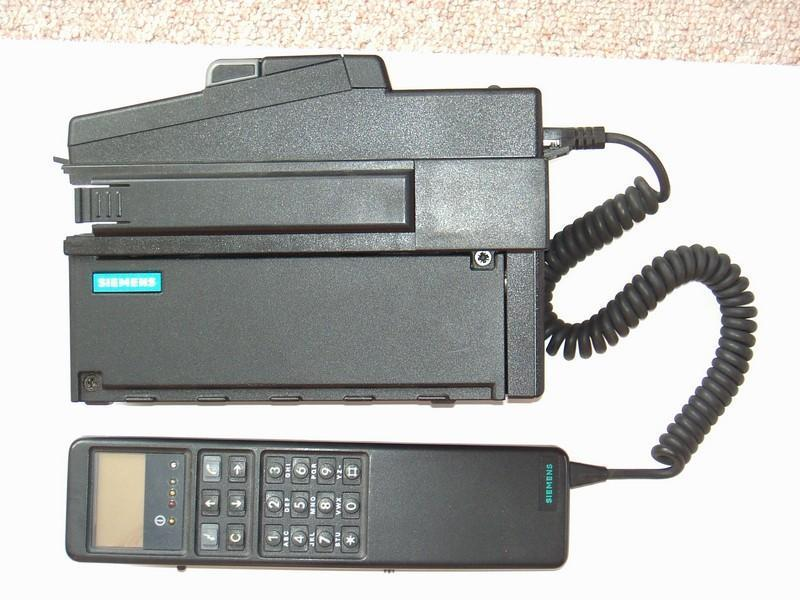
\includegraphics[width=\linewidth]{Kapitel/C-Netz/Grafiken/SiemensC1.jpg}
\captionof{figure}{Mobiltelefon~\cite{c-netz.8}}
\label{fig:c-netz.mobiltelefonZwei}
\end{Figure}
Auch auf Seeschiffen in Küstennähe Deutschlands war ein C-Netz-Gerät an Bord lange weiter verbreitet. Während der Zeit der deutschen Wiedervereinigung 1990 konnten westdeutsche Besitzer von C-Netz-Telefonen bei Aufenthalten in Ostberlin ihr Telefon benutzen und ersparten sich die zeitraubende Zuweisung eines Ferngespräches im DDR-Festnetz~\cite{c-netz.3}.
Der Betrieb des C-Netzes, das am 1. Mai 1985 startete, wurde am 31. Dezember 2000 eingestellt, mit Ausnahme einiger Funkzellen an der deutsch-niederländischen Grenze, die noch einige Monate weiterbetrieben wurden.


\subsection*{Ausblick}
Die Frequenzen des C-Netzes sollen in Zukunft für Railnet (Internet im Zug) genutzt werden. Die Telekom, die das C-Netz bis ins Jahr 2000 betrieb, ist mit ihrer Tochter Telekom Deutschland bei Railnet vertreten. Für die Versorgung im Zug wird WLAN verwendet. Die Verbindung zwischen Zugserver und den stationären Antennen wird mithilfe von Flarion realisiert. Die Datenübertragungsraten von Flash-OFDM liegen maximal bei 3,2 Mbit/s kumuliert, dabei ergeben sich für den Downlink ca. 2,5 Mbit/s und den Uplink ca. 800 kbit/s. Der große Vorteil gegenüber UMTS (Universal Mobile Telecommunications System) sind die geringen Latenzzeiten von unter 50 Millisekunden und eine integrierte Quality-of-Service-Unterstützung. Somit steht jedem Benutzer im Zug eine Breitbandverbindung zur Verfügung. 
Die nordamerikanische Firma Flarion Technologies ist der Entwickler der Flash-OFDM-Technik. Insgesamt sind rund 150 Stationen von Flarion bundesweit auf Sendung. Damit ist eine Abdeckung der Bahnlinien Dortmund–München und Frankfurt am Main–Hamburg gewährleistet (Stand: November 2010)~\cite{c-netz.3}.
Das praktisch unmögliche Roaming in Netze der Nachbarländer war zugleich ein Hauptgrund für die Entwicklung der nächsten Netztechnologie, die erstmals mit dem D Netz ab 1992 zum Einsatz kam~\cite{c-netz.1}. (Bildquelle:~\cite{c-netz.9}) 
\printbibliography[segment=12,heading=subbibliography]
\end{multicols}
\begin{Figure}
\centering
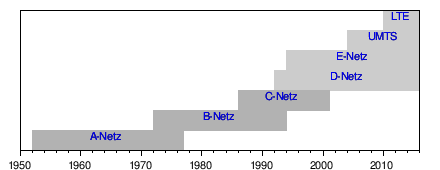
\includegraphics[height=51mm]{Kapitel/C-Netz/Grafiken/ZeitstrahlWiki.png}
\captionof{figure}{Zeitstrahl von A-Netz bis LTE~\cite{c-netz.9}}
\end{Figure}
\newpage